\section{Processing Subsystem Evaluation}
\label{sec:processing_app}
The proposed preprocessing subsystem is responsible for receiving the raw radar data from the AWR2242 
radar chips, depicted in Figure \ref{fig:AWR2243},
and preparing the data for detection. An instance of the subsystem runs per incoming video stream. 
Before outputting the data to the aggregator subsystem which is upstream of the detection and 
tracking subsystem. The subsystem performs the following operations sequentially: formatting, windowing, FFT, and 
integration, (see Figure \ref{fig:preprocessing-dataflow}). Below are the implementation and 
experiment details for each of the operations. 

\begin{figure}[htbp]
    \centering
    \incfig[1]{preprocessing_dataflow} 
    \caption[Dataflow for the preprocessing subsystem.]{Dataflow for the preprocessing subsystem. Multiple instances of the subsystem run on
    separate processes, with each instance receiving compressed baseband radar data samples from an
    incoming video stream. Formatting organises samples into contiguous blocks in memory, and discards
    empty chirps. The windowing stage applies a window function to the data to reduce spectral smearing
    in the next stage. The \gls{fft} stage applies a Fourier Transform across fast time into the frequency
    domain, revealing target range. The coherent integration stage sums the complex \gls{fft} values of
    identical pulses within the same frame.} 
    \label{fig:preprocessing-dataflow}
\end{figure}

\begin{figure}
    \centering
    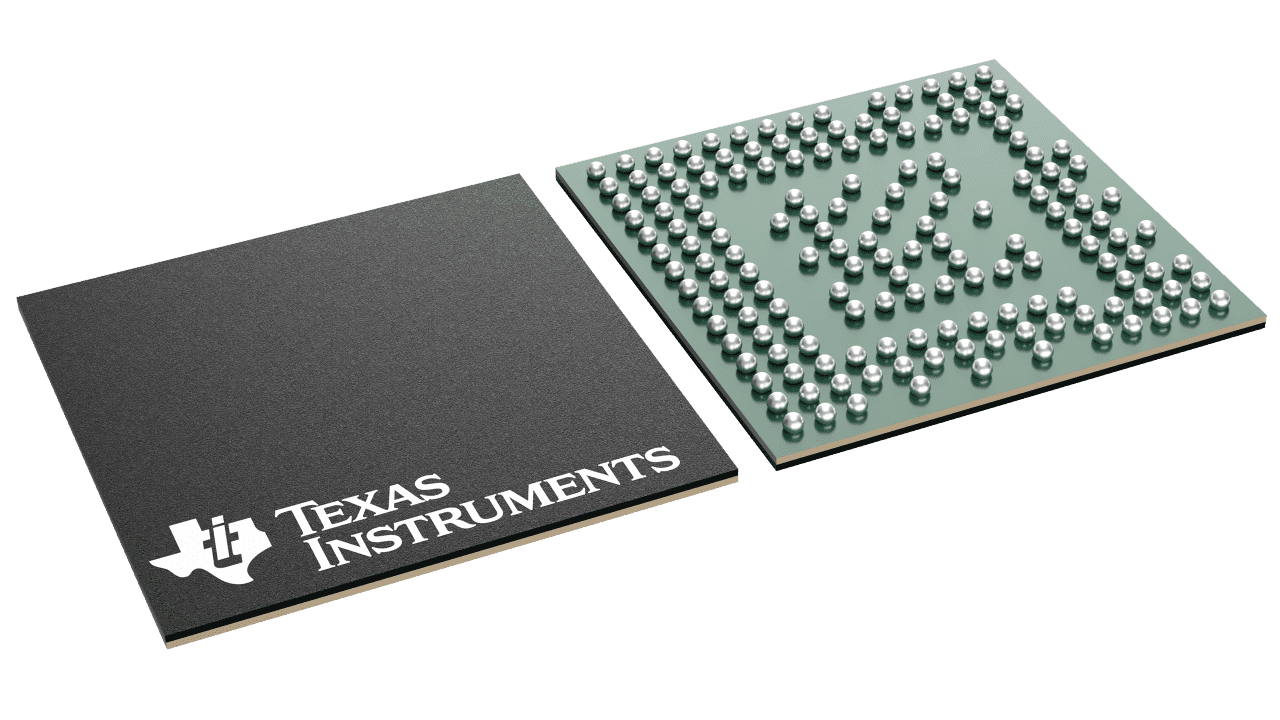
\includegraphics[width=0.5\textwidth]{AWR2243.png}
    \caption[Texas Instruments AWR2243 radar chip.]{Photo of the Texas Instruments AWR2243 radar chip, which is
    used in the radar module. The chip has 3 transmitters and 4 receivers, and outputs the radar data over a CSI
    video stream. The chip is only 10.4mm x 10.4mm, making it suitable for placement on UAV PCBs.}
    \label{fig:AWR2243}
\end{figure}

\subsection{Windowing}
To reveal target range from a single radar pulse, an \gls{fft} is applied to the
de-chirped pulse. 
% The  assumes the finite signal repeats periodically, so when the signal does
% not start and end at the same value, the implicit periodicity introduces a discontinuity. This
% causes energy from a true frequency to spread into adjacent bins — a phenomenon known as spectral
% leakage.

When an \gls{fft} is performed on a finite signal, it is implicitly multiplied by a rectangular window.
A term-wise multiplication in time corresponds to a convolution in the frequency domain, and the
rectangular window's sinc-shaped frequency response has large sidelobes that spread energy from
each frequency bin into its neighbours. By applying a more suitable window function prior to the
FFT, spectral leakage can be reduced, as shown in Figure \ref{fig:hann filter}.

\begin{figure}[htbp]
    \centering
    \includesvg[width=0.6\linewidth]{Images/ffts1}
    \caption[FFT with and without a Hann window showing spectral leakage reduction.]{Results of an \gls{fft} performed on a signal with two frequencies and Gaussian noise, with
    and without a Hann window. Without the Hann window, the bins close to the peak frequency bins 40
    and 45 are significantly elevated due to spectral leakage from those peaks, which would cause
    nearby bins to be falsely detected as targets.}
    \label{fig:hann filter}
\end{figure}

This thesis evaluates a range of practical window functions and their implementation on CPU and GPU. 
Candidate windows include common real-time tapers such as Hann and Hamming, lower-sidelobe windows 
such as Blackman and Blackman--Harris, and adjustable-parameter windows such as Kaiser, which allow 
explicit control over sidelobe level and mainlobe width. Because windowing is a point-wise 
multiplication, it is naturally suited to single instruction, multiple data (SIMD) execution. These 
implementations are compared for their resulting spectral behaviour. 

The sidelobe attenuation and resolution loss are compared for each window and a trade off analysis 
is performed to determine when each window is the most suitable. These procedures provide a basis 
for selecting windows that are spectrally well behaved, sensitive, and 
positively affect the ending track quality. 

\subsection{Integration}
Coherent integration is compared with non coherent integration for their resulting SNR 
improvement, angle estimation quality, and track quality on real and simulated data. 
The relationship between coherent integration window size and the performance metrics 
is also explored. 

After, the latency and throughput of coherent integration is characterised in relation to
the other stages, and the integration window size. The trade off analysis is 
between SNR and latency is performed. The integration stage is also evaluated in the
ablation study of the processing application. 